\documentclass{article}

\usepackage{graphicx}
\usepackage[utf8]{inputenc}
\usepackage[T1]{fontenc}

\begin{document}

\title{Predictive Models for Water Demand and Population Growth in the capital area of Iceland}
\author{Sigurdur Haukur Birgisson}

\maketitle

\begin{abstract}
    This research paper presents the development and performance evaluation of predictive models for water demand and population growth in the capital area of Iceland. The models utilize data provided by Reykjavik Energy and leverage machine learning algorithms, including XGBoostRegressor and RandomForestRegressor. The study aims to provide valuable insights for resource planning, infrastructure investment, and sustainable development in the water industry. The results demonstrate promising predictive capabilities within the limitations of the available dataset.
\end{abstract}

\tableofcontents
\newpage

\section{Introduction}
The water industry plays a crucial role in ensuring sustainable water management practices. Accurate predictions of water demand and population growth are essential for efficient resource allocation and infrastructure planning. This research focuses on developing predictive models to address these challenges in Reykjavik, Iceland.

\section{Data}
The data used in this study was available on Gagnagatt, the open data portal of the Icelandic government, it was collected from Reykjavik Energy (the main company serving water to people in the capital area of Iceland). The hot water \cite{hot-water} and cold water \cite{cold-water}. The datasets contain annual records of water demand, population growth, and related variables. Data from the Icelandic Meterological Office \cite{weather} was also used.

All the datasets were joined into one, on the year variable. The data was then split into a training set (80\%) and a test set (20\%). The training set was used to train the models and the test set was used to evaluate the performance of the models.

A correlation matrix was created to identify the most important variables. The correlation matrix is shown in Figure \ref{fig:correlation-matrix}.

\begin{figure}[!hb]
    \centering
    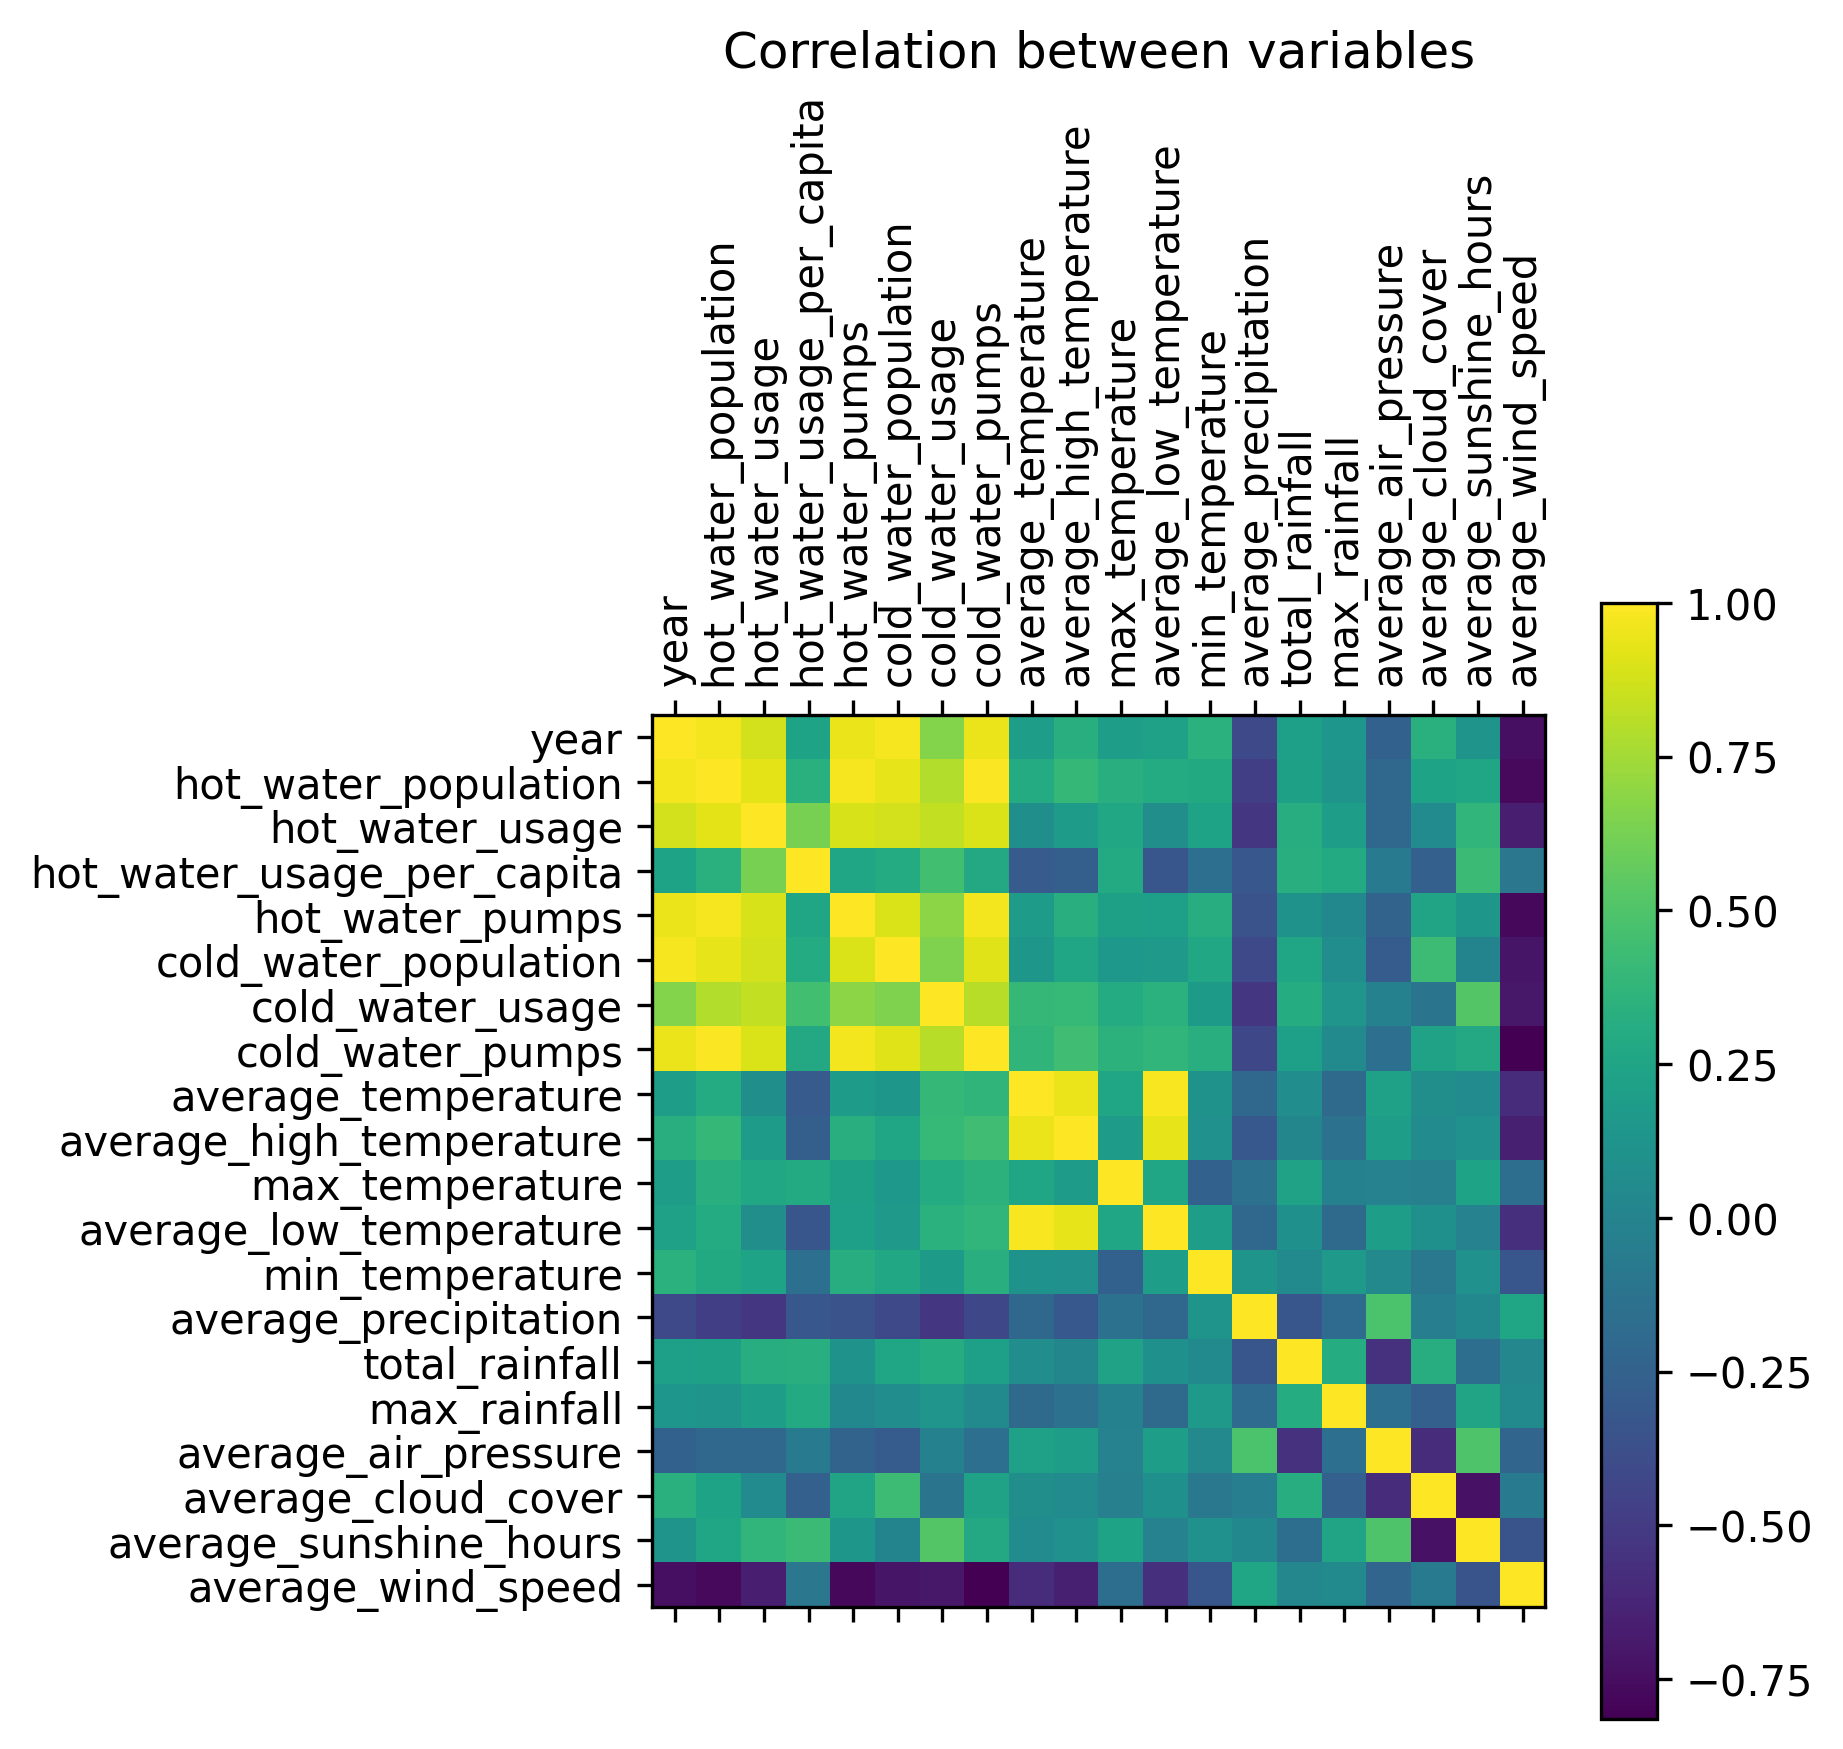
\includegraphics[width=0.7\textwidth]{../figures/correlation.png}
    \caption{Correlation matrix}
    \label{fig:correlation-matrix}
\end{figure}

The correlation matrix shows that the most important variables relating to water demand are the number of people living in the area (e.g. hot\_water\_population), the year (e.g. year), and the average min temperature (e.g. average\_temperature). However, the average min temperature has little correlation compared to the other two, so it was not used to predict water demand.

\section{Methods}
The models were trained on the training set and evaluated on the test set. The performance of the models was evaluated using the mean absolute error (MAE), the root mean squared error (RMSE), and validation accuracy.

Before deciding on the kind of model to use, the trends in the data were analyzed. The trends are shown in Figure \ref{fig:water-demand-trends} and Figure \ref{fig:population-trends}.

\begin{figure}[h]
    \centering
    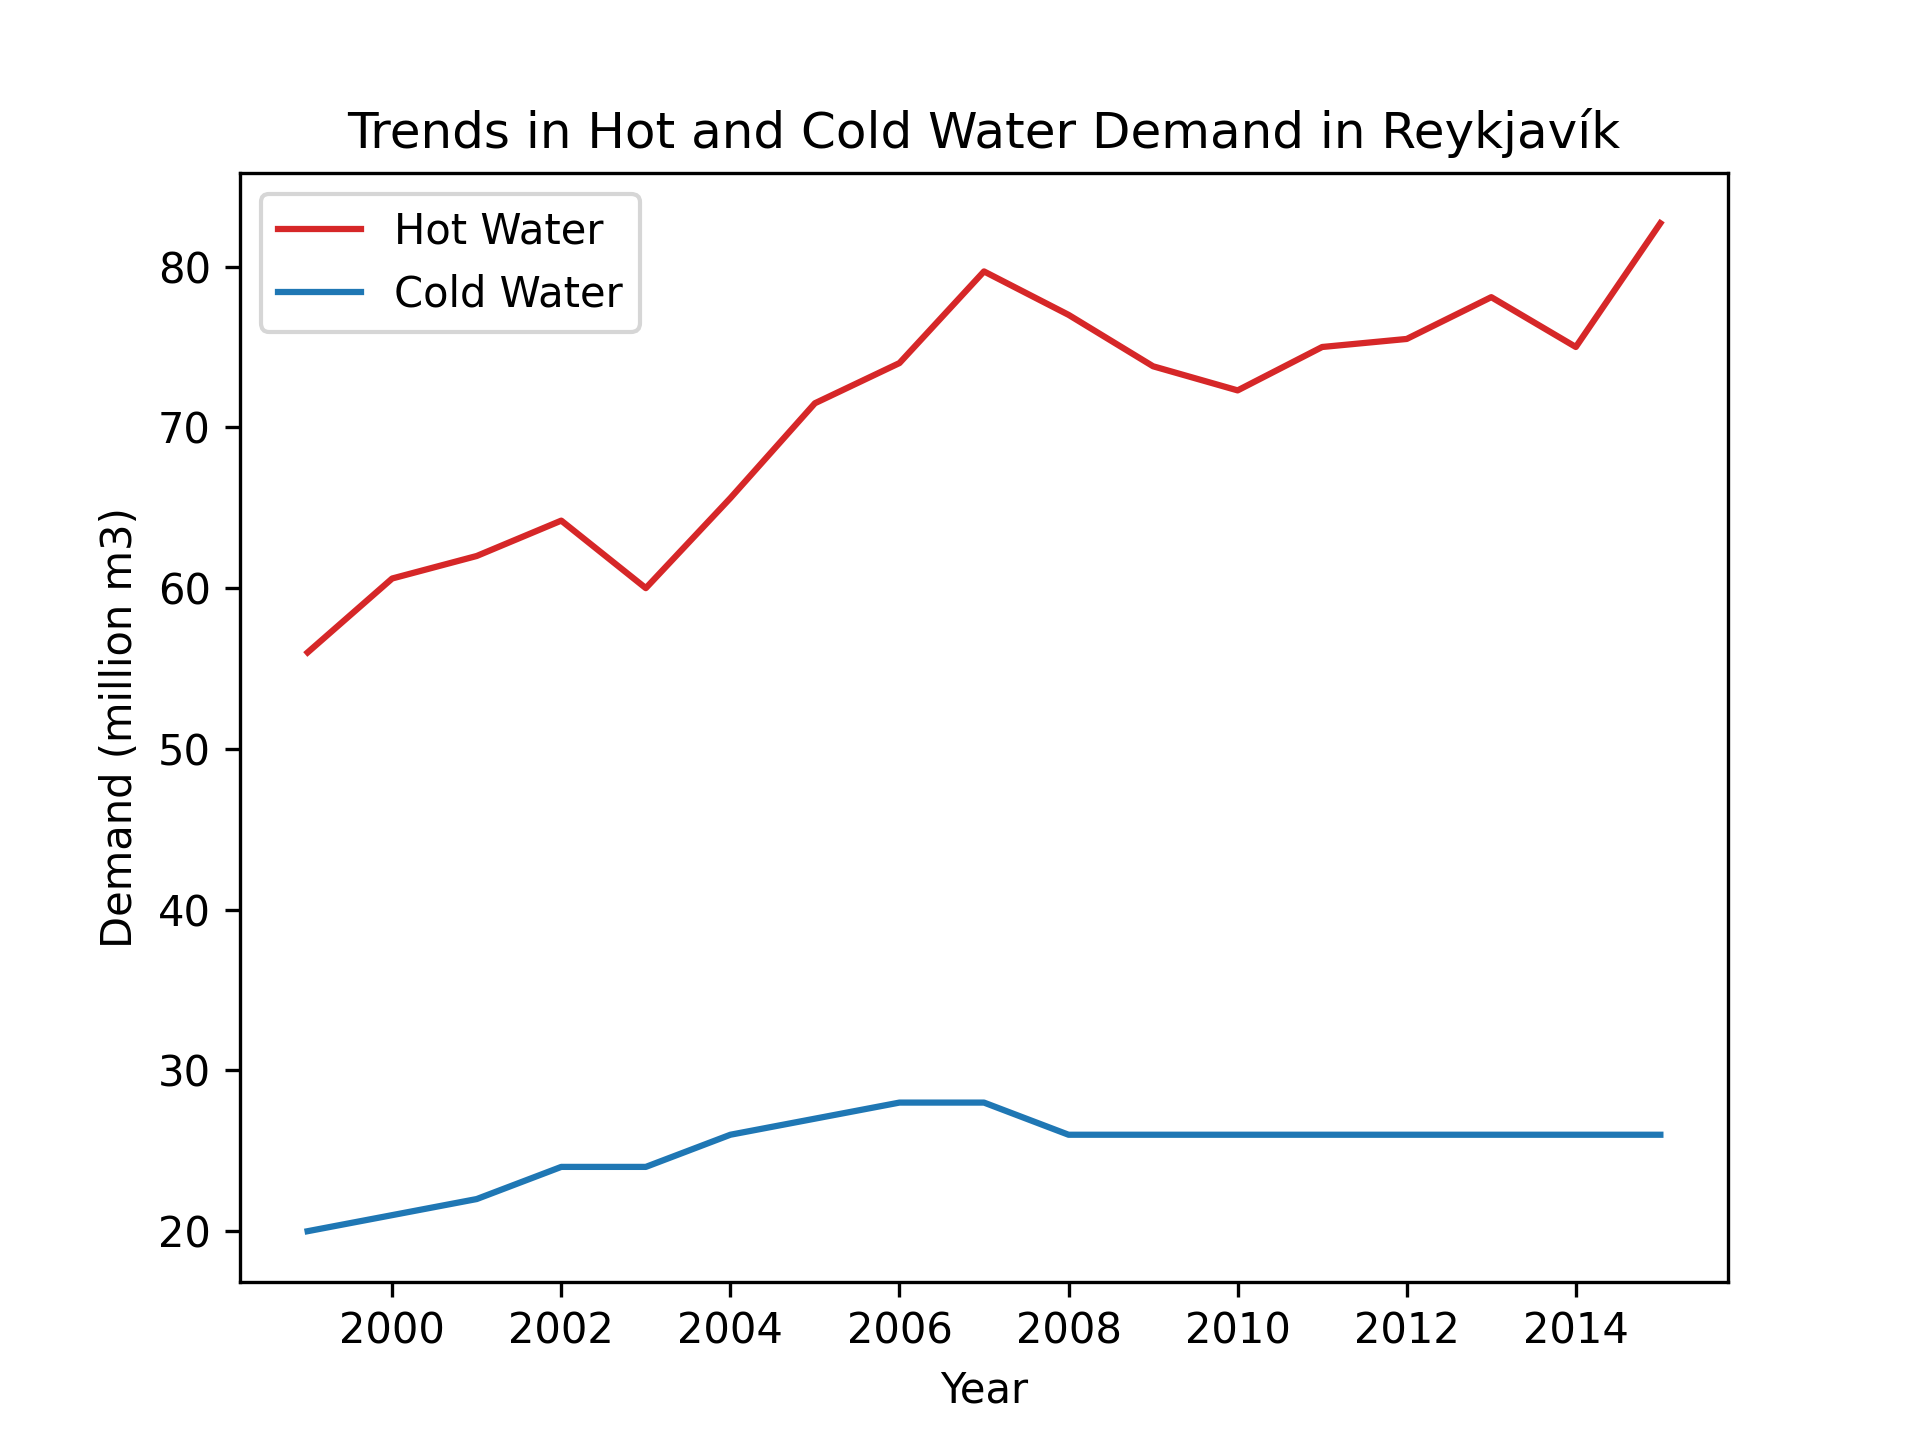
\includegraphics[width=0.8\textwidth]{../figures/trends-in-hot-and-cold-water-demand.png}
    \caption{Water demand trends}
    \label{fig:water-demand-trends}
\end{figure}

\begin{figure}[!h]
    \centering
    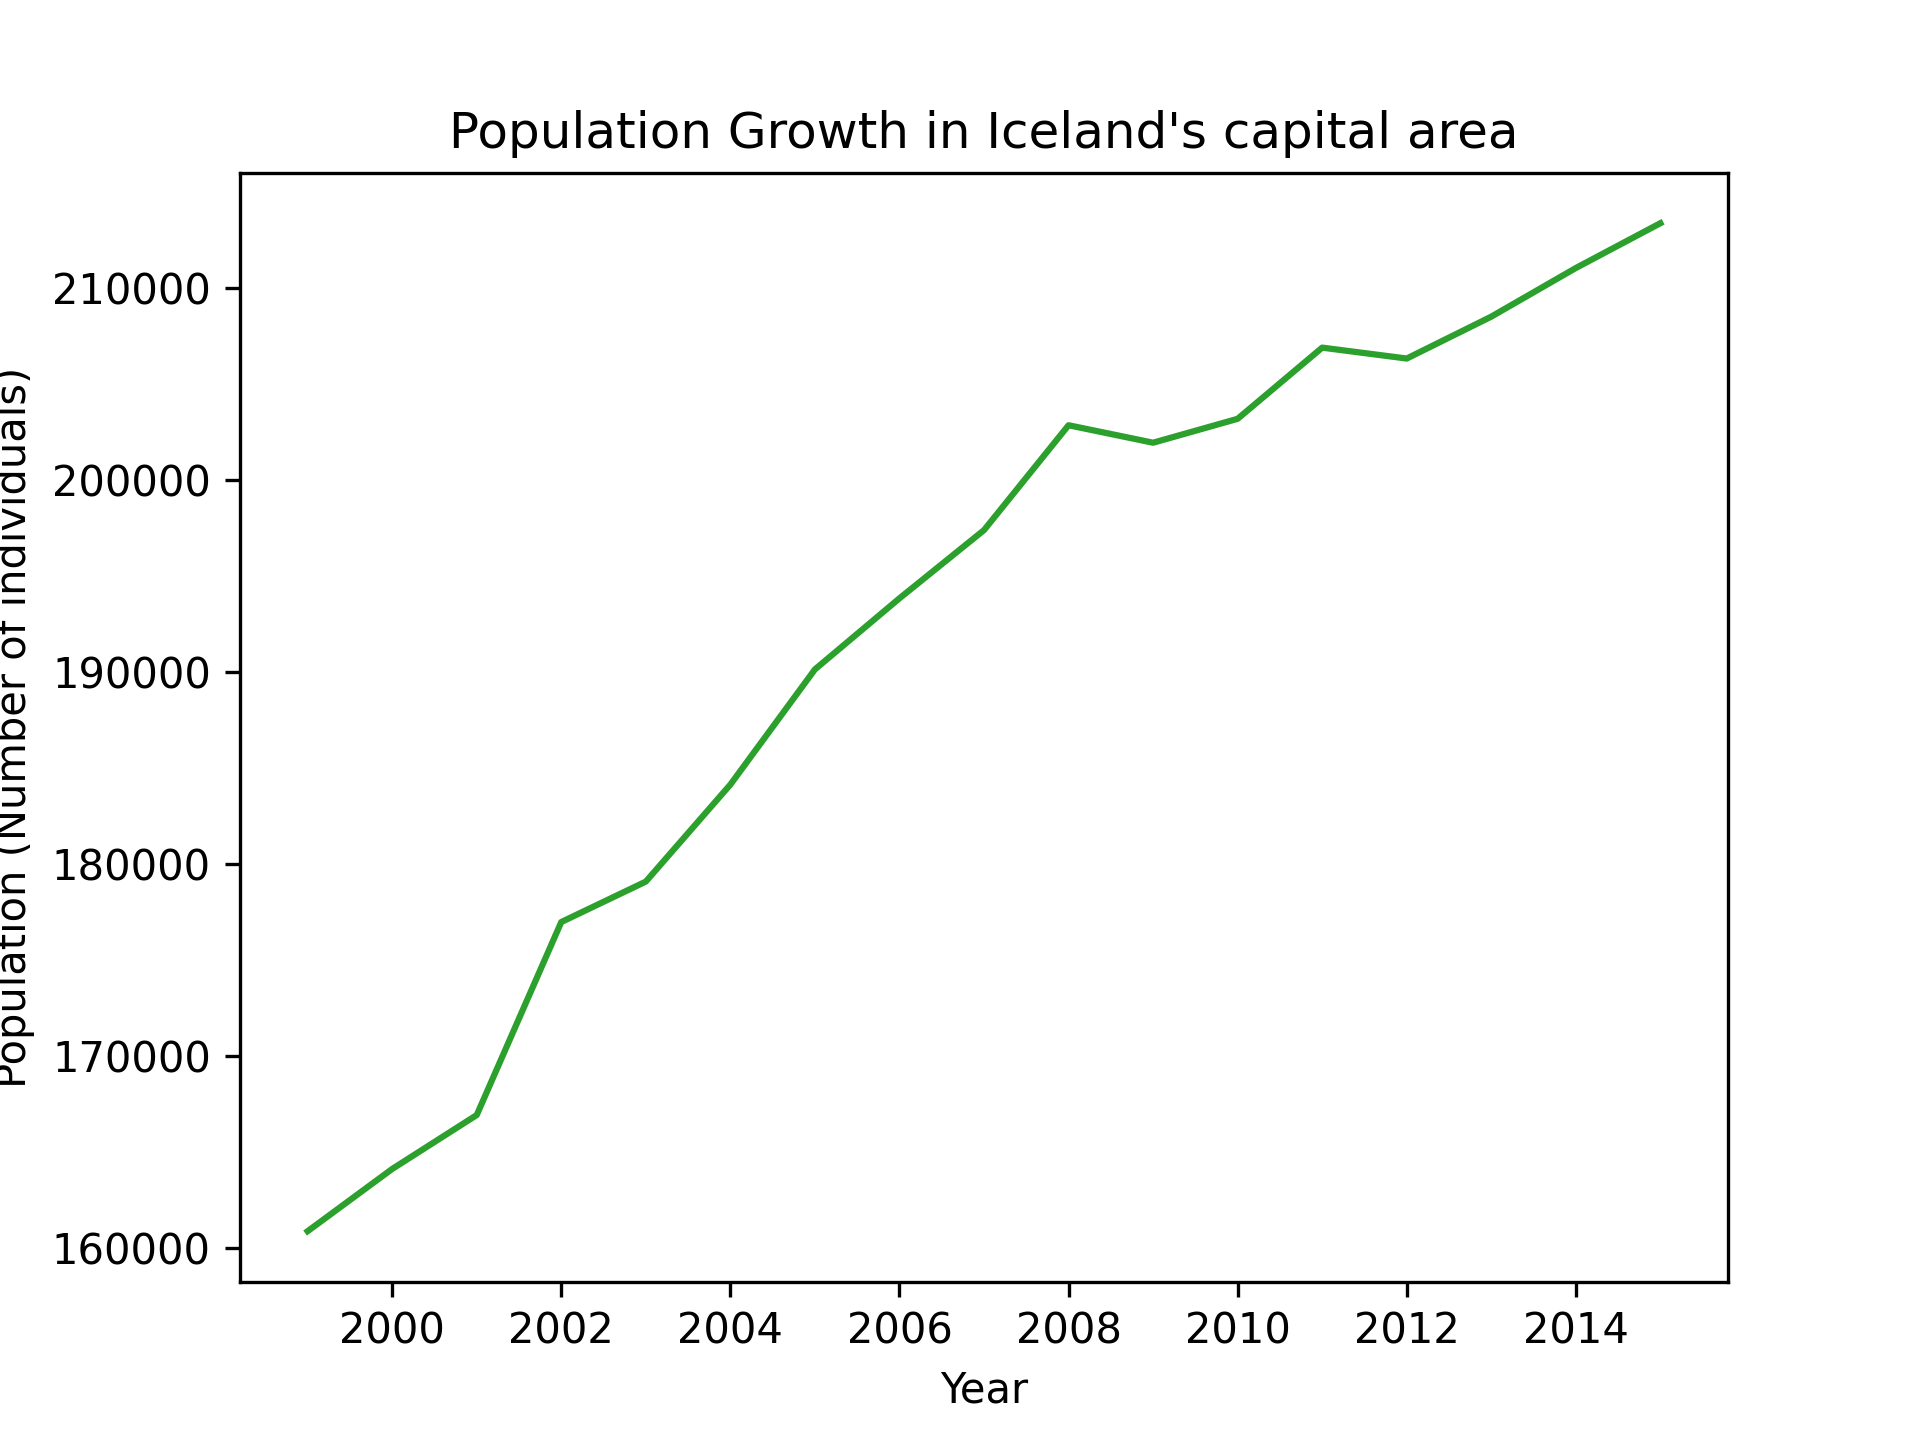
\includegraphics[width=0.8\textwidth]{../figures/population-growth.png}
    \caption{Population trends}
    \label{fig:population-trends}
\end{figure}

The trends show that water demand and population growth are increasing linearly over time, with some noise in the data, especially in the data for hot water.

The models used in this study are XGBoostRegressor and RandomForestRegressor, since they can handle small datasets and are good at predicting time series data.

\newpage

\section{Results}
The results of the models are shown in Table \ref{tab:results}. The validation accuracy represents the model's performance on unseen data during the validation phase. It is a measure of how well the model predicts outcomes compared to the actual values (the highest value is 1). The MSE, RMSE, and MAE are common metrics used to evaluate regression models. The MSE calculates the average squared difference between predicted and actual values, the RMSE is the square root of the MSE, and the MAE measures the average absolute difference between predicted and actual values. The lower the values of these metrics, the better the model.

\begin{table}[!ht]
    \centering
    \begin{tabular}{llll}
        \hline
        ~                   & hot water model & cold water model & population model \\ \hline
        validation accuracy & 0.76            & 0.91             & 0.96             \\
        MSE                 & 0.22            & 0.12             & 0.01             \\
        RMSE                & 0.47            & 0.34             & 0.06             \\
        MAE                 & 0.42            & 0.32             & 0.05             \\ \hline
    \end{tabular}
    \caption{Results}
    \label{tab:results}
\end{table}

The results show that the models are able to predict water demand and population growth with reasonable accuracy. The models for cold water and population growth perform better than the model for hot water. This is likely due to the noise in the data for hot water, as shown in Figure \ref{fig:water-demand-trends}.

\begin{figure}[!ht]
    \centering
    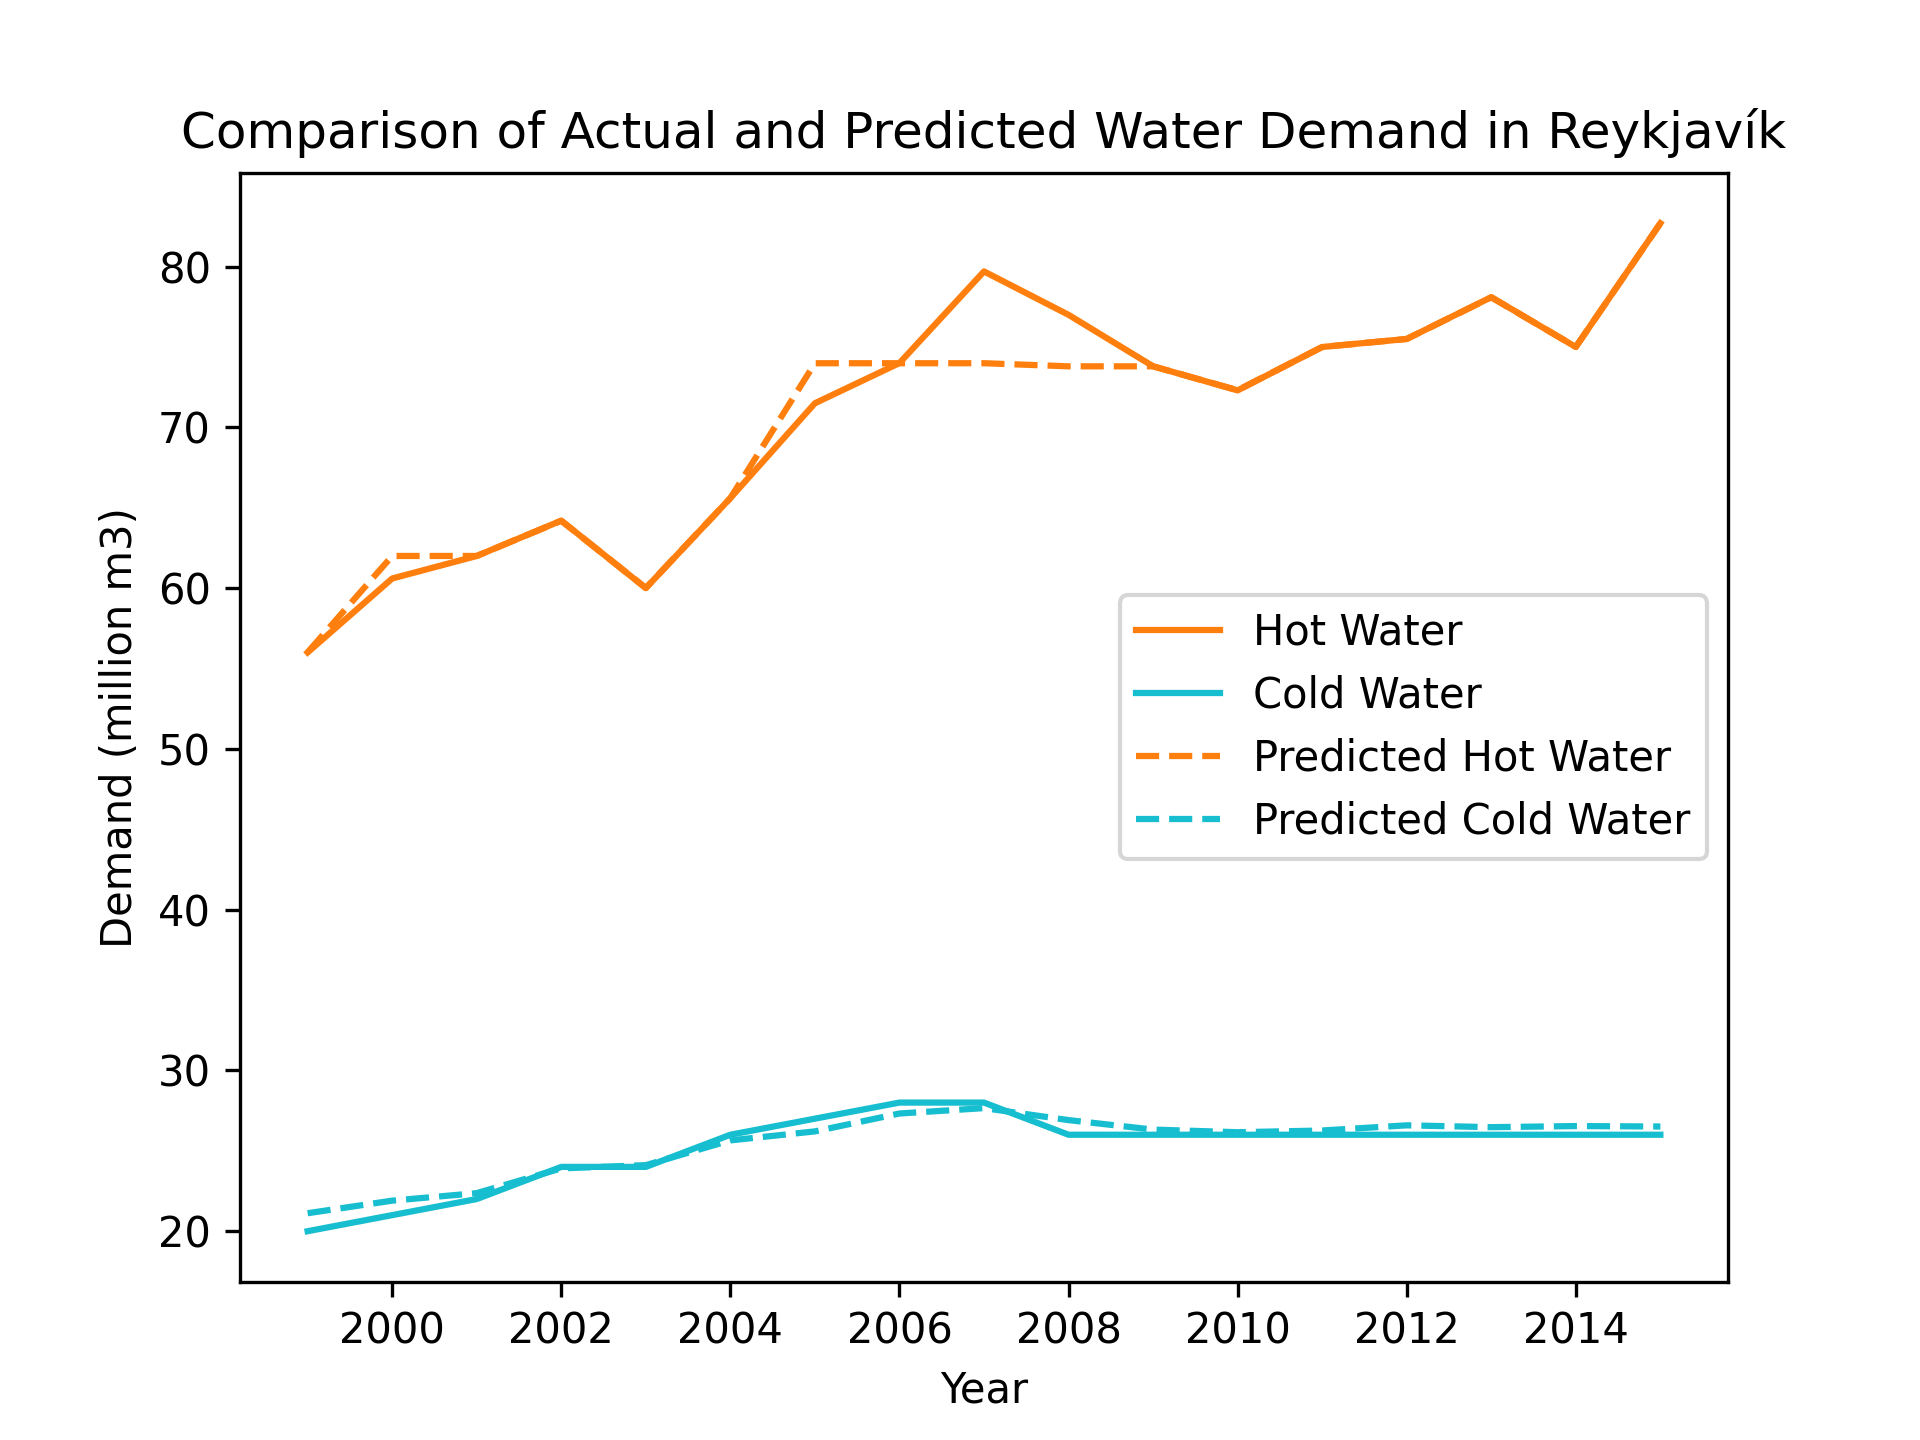
\includegraphics[width=0.8\textwidth]{../figures/comparision-of-actual-and-predicted-water-demand.png}
    \caption{Predictions of water demand}
    \label{fig:water-demand-predictions}
\end{figure}

\begin{figure}[!hb]
    \centering
    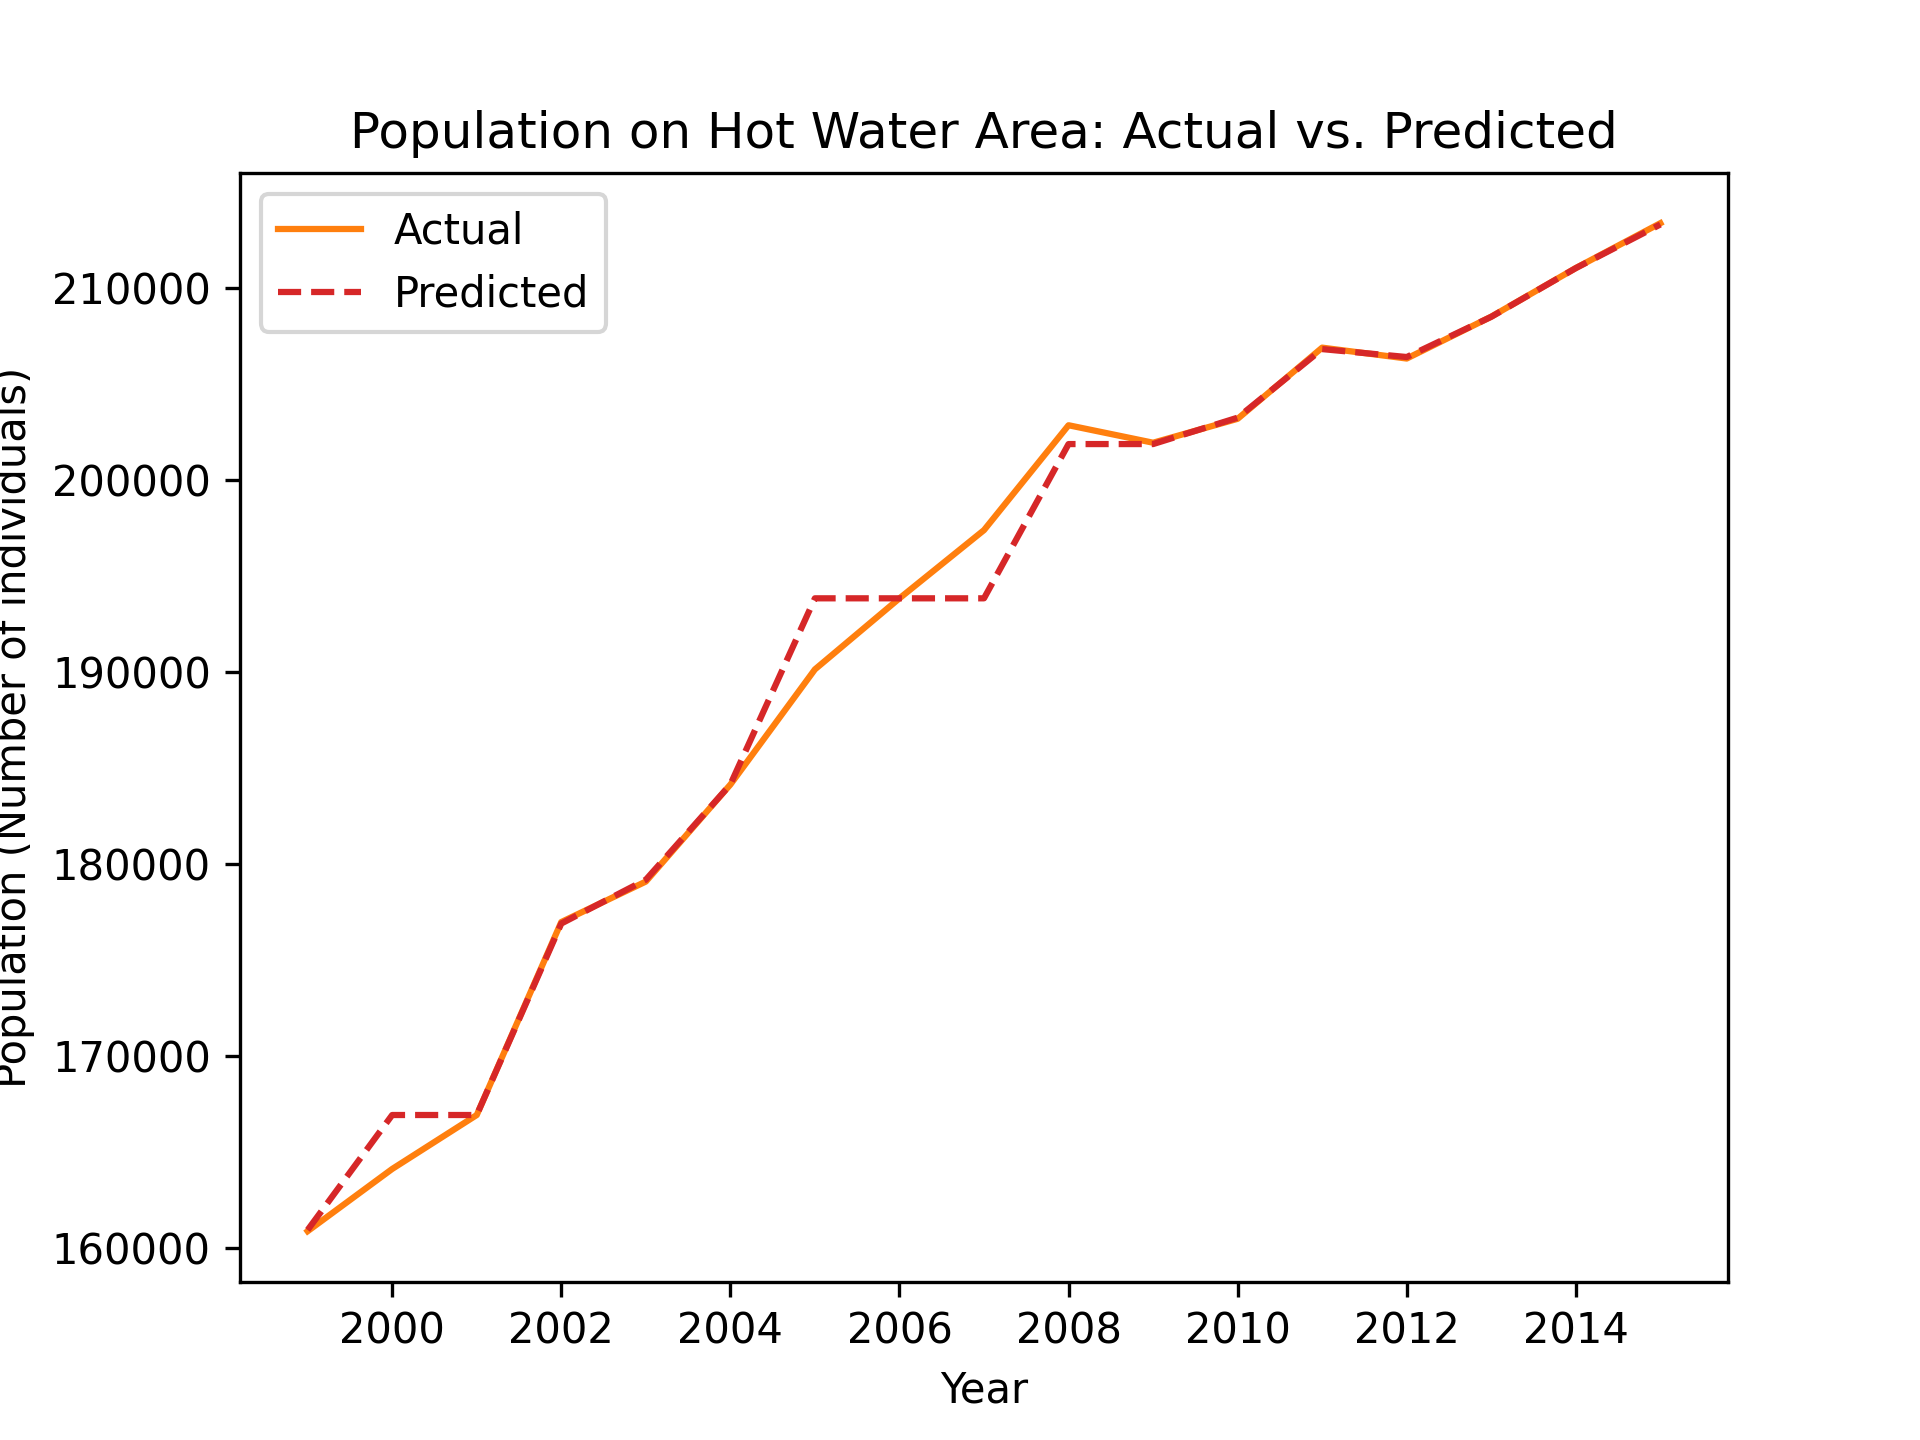
\includegraphics[width=0.7\textwidth]{../figures/population-hot-water-area-actual-vs-predicted.png}
    \caption{Predictions of population growth}
    \label{fig:population-predictions}
\end{figure}

Plotting the predictions against the actual values shows that the models are able to capture the trends in the data, as shown in Figure \ref{fig:water-demand-predictions} and Figure \ref{fig:population-predictions}.

\newpage

\section{Discussion}
The results of this study indicate that the developed predictive models for water demand and population growth in the capital area of Iceland show promising capabilities. However, it is important to note that the dataset used in this study consisted of only 16 data points since it was collected annually from 1999 to 2015. The limited number of data points may affect the generalizability of the models and their ability to capture complex patterns and variations.

Despite the small dataset, the models demonstrated reasonable accuracy in predicting water demand and population growth. They were able to capture the overall increasing trends in both water demand and population over time(continued):

as evidenced by the linear patterns observed in the data. However, it's crucial to interpret the results with caution and acknowledge the limitations imposed by the small dataset.

The predictive models developed in this study have various applications in the water industry and urban planning. Accurate predictions of water demand can assist in efficient resource allocation, infrastructure planning, and optimization of water distribution systems. By forecasting future water demand, water utilities can better anticipate and respond to fluctuations in demand, ensuring a stable water supply for the population.

Furthermore, these predictive models can aid in long-term planning for sustainable water management. By understanding future population growth and its impact on water demand, policymakers can make informed decisions regarding infrastructure development, conservation strategies, and water resource allocation. The models provide valuable insights for decision-makers to develop effective policies, ensure sustainable development, and address potential challenges associated with population growth and changing water demand patterns.

However, it is important to recognize that these predictive models have limitations. The small dataset used in this study may not fully capture the complexities and dynamics of water demand and population growth. Additionally, external factors such as economic conditions, climate change, and societal changes could influence water demand and population patterns, which were not explicitly considered in this study. Future research could incorporate more comprehensive datasets and explore the inclusion of additional variables to improve the accuracy and robustness of the predictive models.

\section{Conclusion}
In conclusion, this research paper presented the development and performance evaluation of predictive models for water demand and population growth in the capital area of Iceland. Despite the limited dataset consisting of only 16 data points from 1999 to 2015, the models demonstrated promising predictive capabilities.

The developed models have various applications in resource planning, infrastructure investment, and sustainable development in the water industry. They can assist decision-makers in optimizing water distribution systems, anticipating future water demand, and addressing challenges associated with population growth.

However, it is important to acknowledge the limitations of the models due to the small dataset and the potential influence of external factors. Further research is needed to refine and validate the models using more comprehensive datasets and to explore the inclusion of additional variables to enhance their accuracy and applicability.

The findings of this study contribute to the understanding of water demand and population growth patterns in the capital area of Iceland, providing valuable insights for decision-makers in the water industry and urban planning.

\bibliographystyle{plain}
\bibliography{mybib}

\end{document}
